本部分以windows11系统为例进行安装说明,如有使用特殊体质mac系统还请寻找其他方法(也许后续会补充进来)。
安装双系统主要分为以下四个流程:windows系统分区,制作启动盘,从U盘进行安装,系统设置相关。下面将进行一一说明。
\subsubsection{windows系统分区}
右键桌面上的“此电脑”图标,点击“管理”选项,进入“磁盘管理”界面,在这里你会看到电脑上存在若干个磁盘分区如下图所示。

\begin{figure}[H]
    \centering
    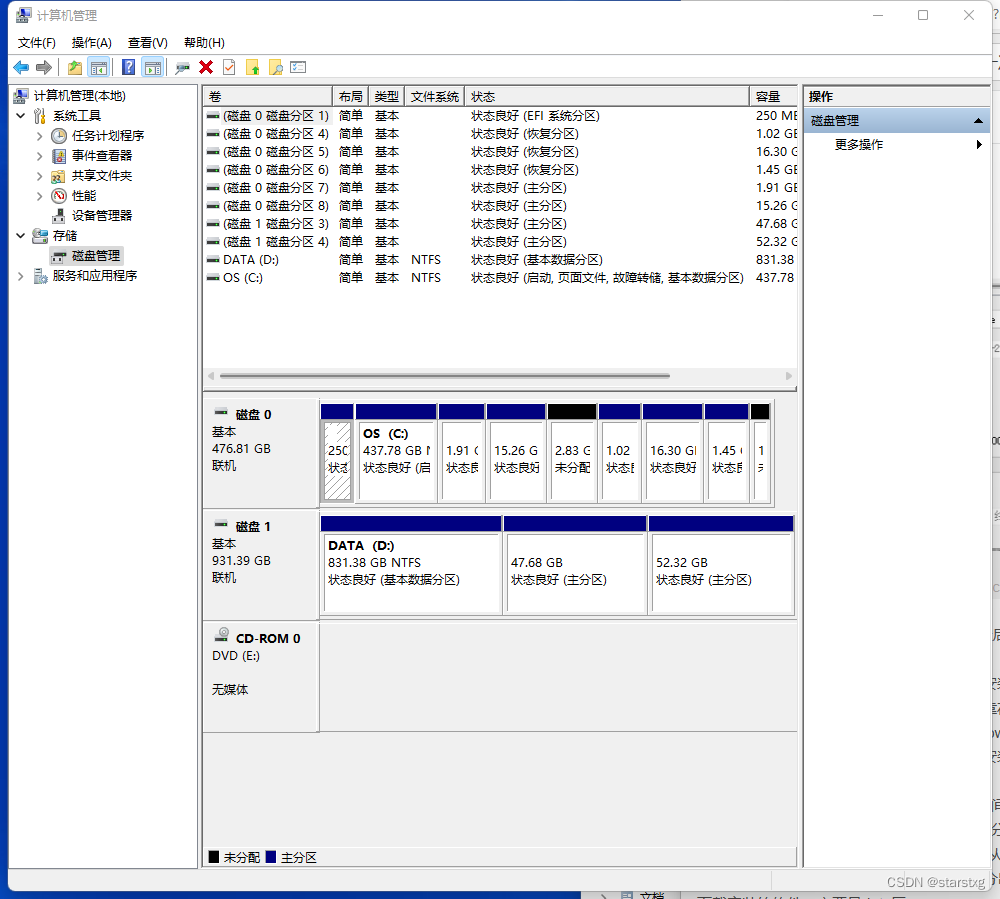
\includegraphics[width=0.7\textwidth]{linux1.png}
    \caption{磁盘分区} % 图片标题
    \label{fig:linux1} % 图片标签,用于引用
\end{figure}

选择一个剩余空间较大的磁盘,右击,点击“压缩卷”,等待计算完成后会显示当前磁盘中可用的压缩空间大小。输入你要留给ubuntu系统的空间量(注意是以MB为单位的),推荐是预留200G,后续内存不够虽然可以扩容但操作起来有点麻烦。

\begin{figure}[H]
    \centering
    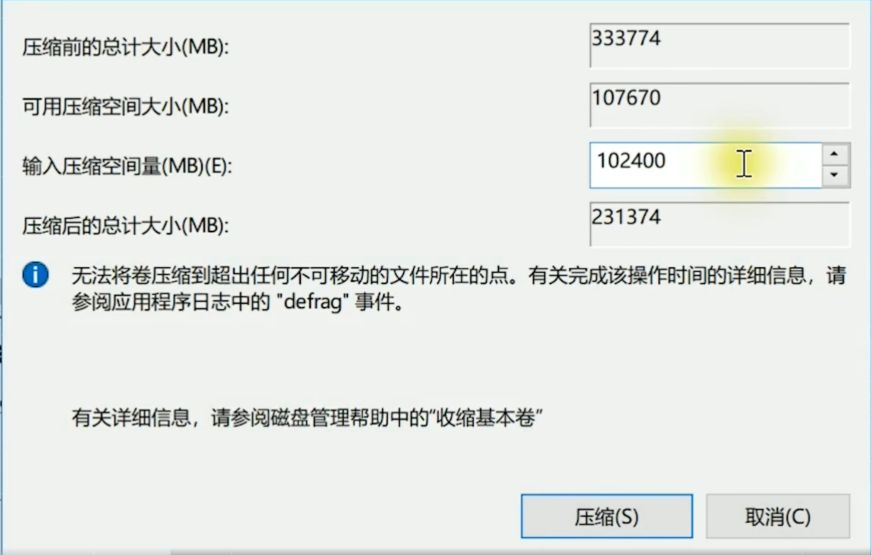
\includegraphics[width=0.7\textwidth]{linux2.jpg}
    \caption{分配linux空间} % 图片标题
    \label{fig:linux2} % 图片标签,用于引用
\end{figure}

输入好后点击“压缩”,压缩完成后出现一个“未分配”的区域则说明分区完成。

\subsubsection{制作启动盘}
首先需要一个内存大于16GB的U盘,请先对其中的文件进行备份,后续操作需要格式化这个U盘。

然后进入ubuntu官网下载ubuntu22.04版本的镜像,下载链接为

\url{https://ubuntu.com/download/alternative-downloads}

注意是下载22.04.5 Desktop!

下载好后还需要下载一个软碟通来将刚刚的ISO写入U盘中,下载链接

\url{https://www.ultraiso.net/xiazai.html} 

打开软碟通点击“继续试用”即可,不需要订购。进入软碟通界面,点击左上角的“文件”-\textgreater“打开”,选择刚刚下载的ISO镜像。点击“启动”-\textgreater“写入硬盘映像”,在弹出窗口的“硬盘驱动器”选项栏中确定是自己现在插上的U盘,写入方式选择USB-HDD+。

\begin{figure}[H]
    \centering
    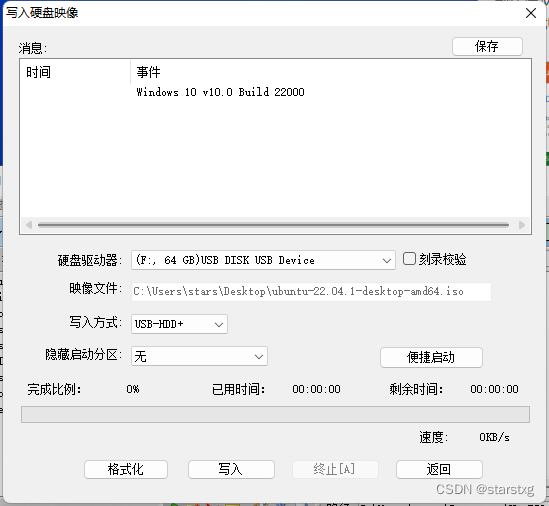
\includegraphics[width=0.7\textwidth]{linux3.png}
    \caption{制作启动盘} % 图片标题
    \label{fig:linux3} % 图片标签,用于引用
\end{figure}

然后对硬盘进行格式化,文件系统选择FAT32(默认),格式化完成后点击“写入”,等待写入完成。

\begin{figure}[H]
    \centering
    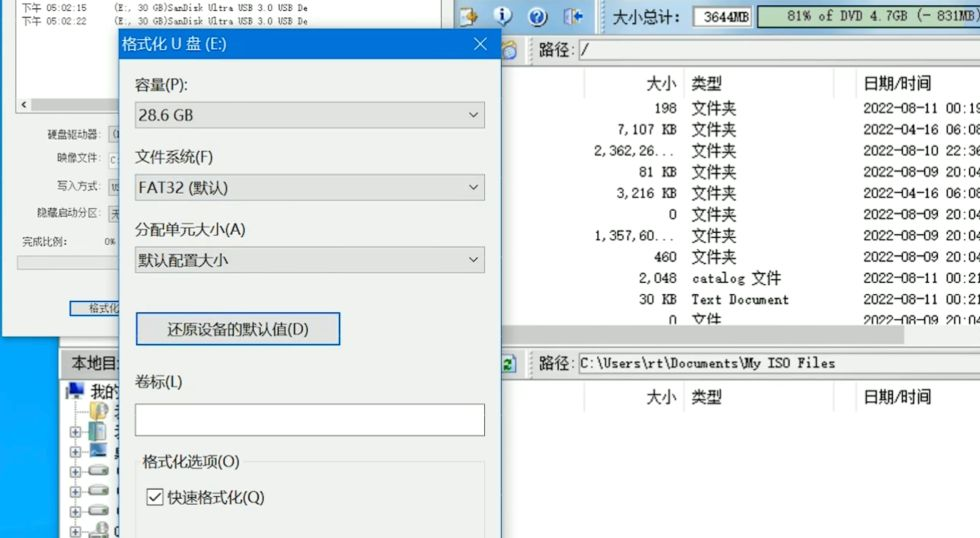
\includegraphics[width=0.7\textwidth]{linux4.jpg}
    \caption{U盘格式化} % 图片标题
    \label{fig:linux4} % 图片标签,用于引用
\end{figure}

U盘被制作成启动盘后仍可以存放其它的文件,插到windows中会提示该U盘有问题建议修复之类的,U盘没坏的话这时候不用管它就好。启动盘被称为“数字生命”,所以请好好保存。
\subsubsection{从U盘进行安装}
插入之前做好的启动盘,重启电脑,重启时快速重复按下启动选项快捷键,各个主板的启动选项快捷键有所不同,可以参考下表进行操作。

\begin{figure}[H]
    \centering
    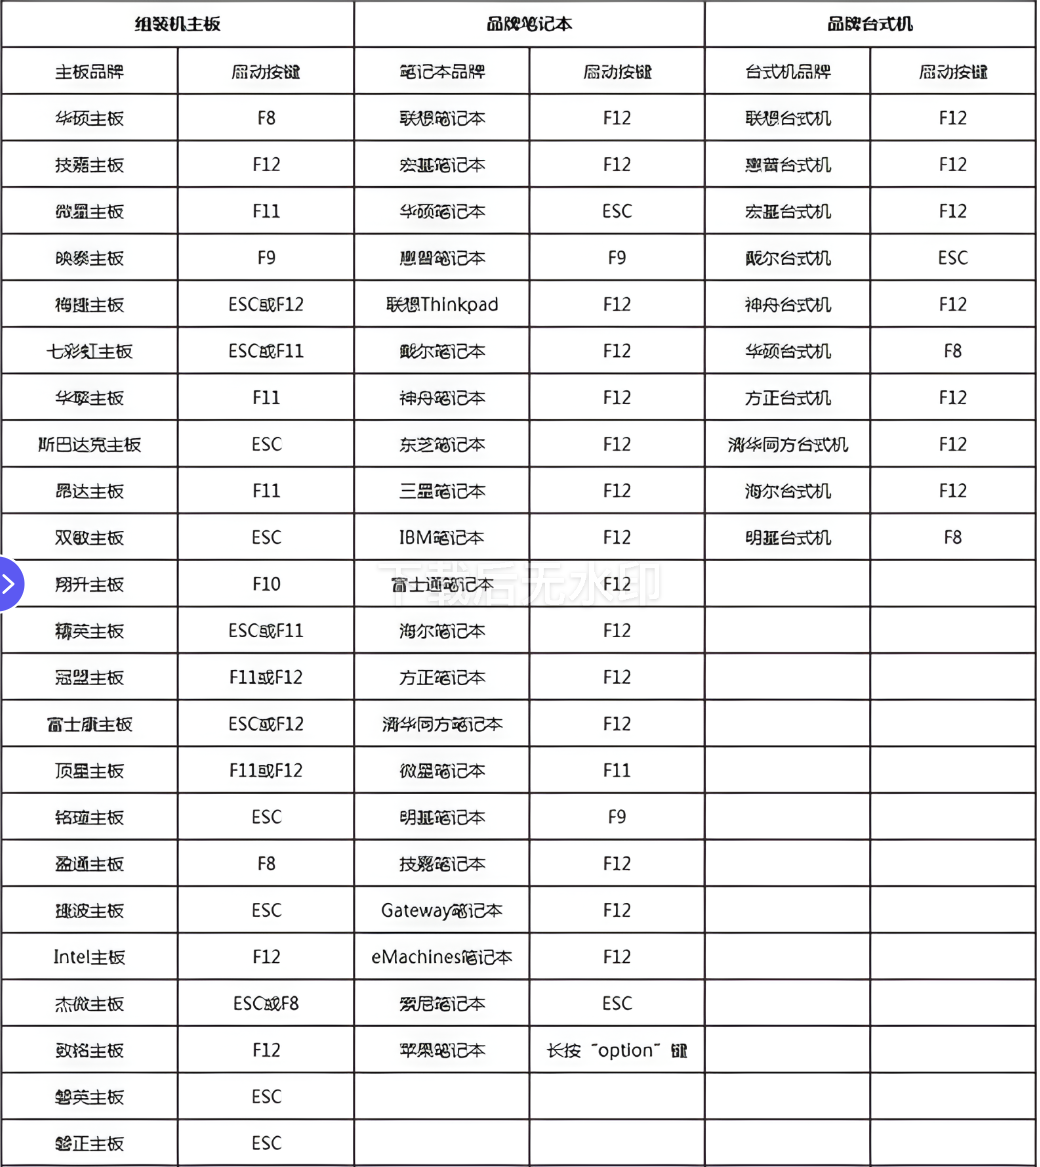
\includegraphics[width=0.7\textwidth]{install1.png}
    \caption{启动选项快捷键一览} % 图片标题
    \label{fig:install1} % 图片标签,用于引用
\end{figure}

进入启动选项界面后通过上下键选择Linpus lite选项,回车,进入系统安装程序,选择Try or Install Ubuntu,再回车,现在你离成功安装ubuntu双系统只有一步之遥啦。

\begin{figure}[H]
    \centering
    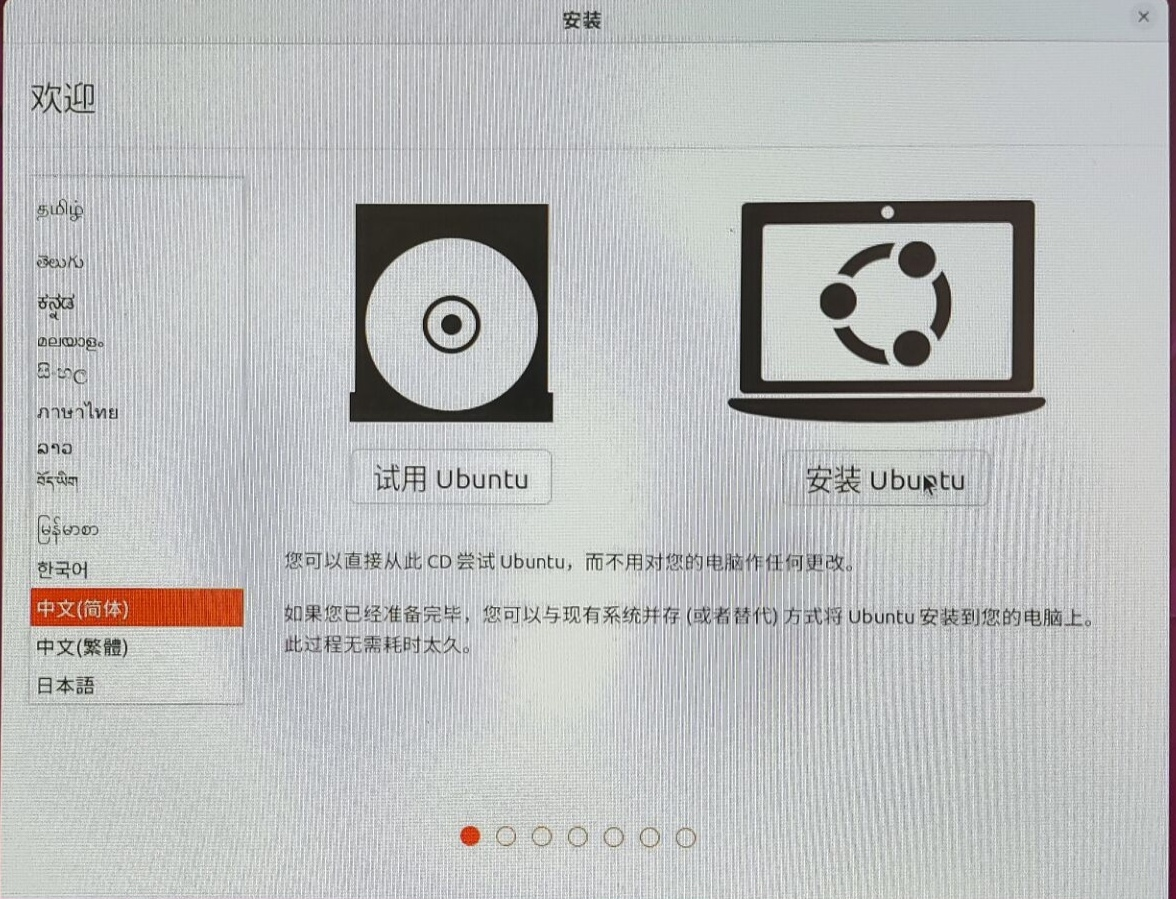
\includegraphics[width=0.7\textwidth]{install2.jpg}
    \caption{开始安装ubuntu} % 图片标题
    \label{fig:install2} % 图片标签,用于引用
\end{figure}

进入安装环节,首先选择语言为简体中文,点击“安装Ubuntu”,“键盘布局”确认是中文就好,下一步无线连接现在不用连。“更新和其他软件”界面选择“正常安装”,勾选“为图形或无线硬件,以及其它媒体格式安装第三方软件”并设置自己用户的密码,注意这个密码后面会经常用到,所以不建议设的过长。

\begin{figure}[H]
    \centering
    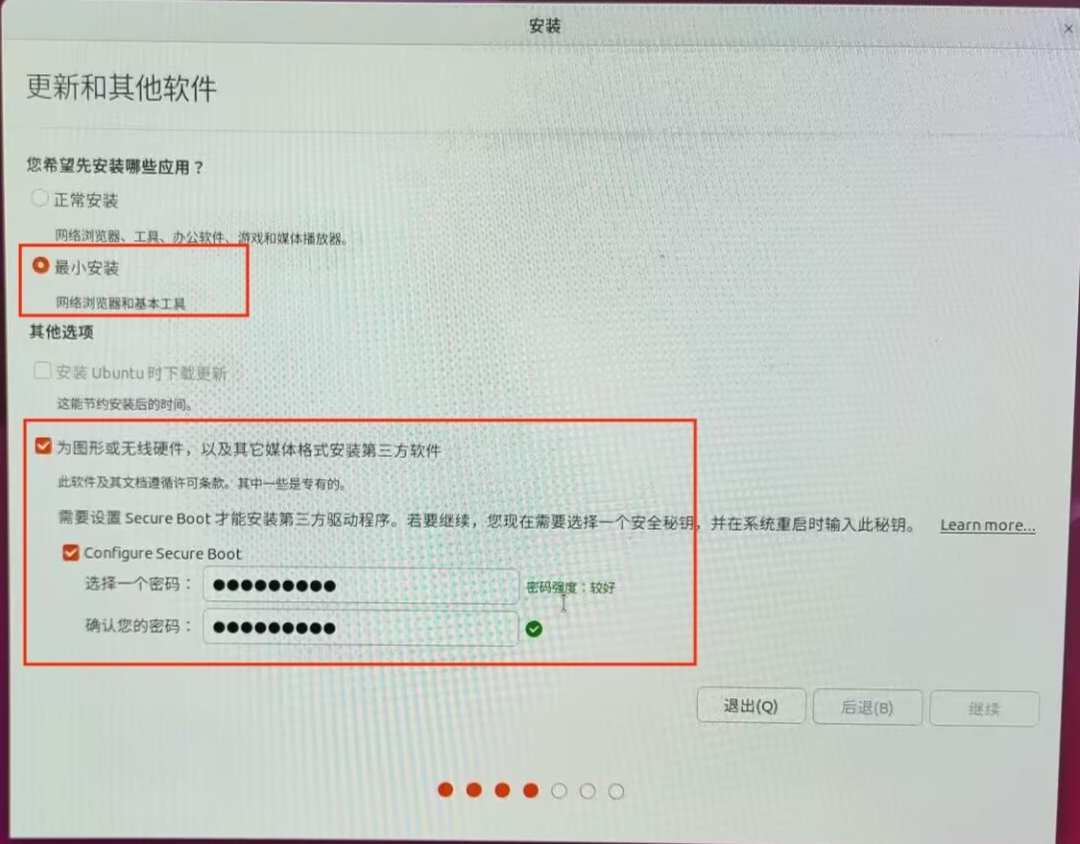
\includegraphics[width=0.7\textwidth]{install3.jpg}
    \caption{设置密码} % 图片标题
    \label{fig:install3} % 图片标签,用于引用
\end{figure}

在下一步“安装类型”中一定一定要选择“其它选项”!!!

然后来到“安装类型”,在这里我们需要创建ubuntu的分区(注意内存大小依然是以MB为单位)并挂载到相应的挂载点上。这里有两种方法:
\begin{enumerate}
	\item \textbf{全部挂载到根目录下}

找到之前压缩出来的空闲区域,双击选项,在弹出窗口的挂载点一栏输入/即可。这种方式最直接、最无脑,适合啥也不明白的新手操作,但是不利于多个分区的内存分配,在备份系统镜像的时候也无法按照不同分区分开备份,因此建议还是按照第二种方法进行分区。
	\item \textbf{挂载到不同目录下}

先分逻辑分区,再分主分区。
	\begin{enumerate}
		\item /boot启动分区:逻辑分区,一般选择200M-2G,放置Ubuntu的启动引导文件。
		\item /swap交换分区(虚拟内存):逻辑分区,一般分16GB就够了。
		\item / 根分区(root分区):逻辑分区,80GB左右差不多。
		\item /home分区:主分区,剩下的内存一起分给/home就好,平时文件也都放这边,要的内存最大。
	\end{enumerate}

点击压缩的空闲区域,点击左下角的加号

\begin{figure}[H]
    \centering
    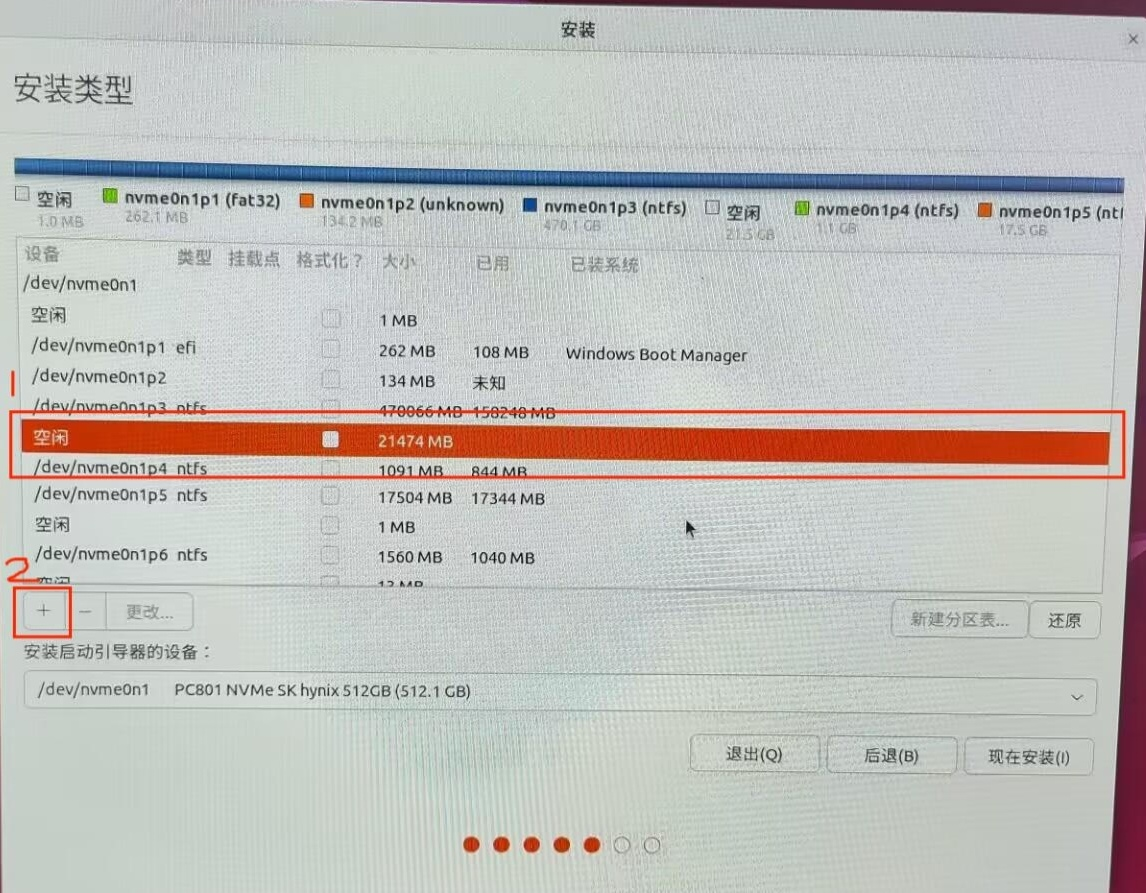
\includegraphics[width=0.7\textwidth]{install4.jpg}
    \caption{选择分区} % 图片标题
    \label{fig:install4} % 图片标签,用于引用
\end{figure}

在弹出的窗口选择大小,新分区类型,新分区位置,文件系统类型,挂载点,依次对/boot,/swap,/,/home进行分区

\begin{figure}[H]
    \centering
    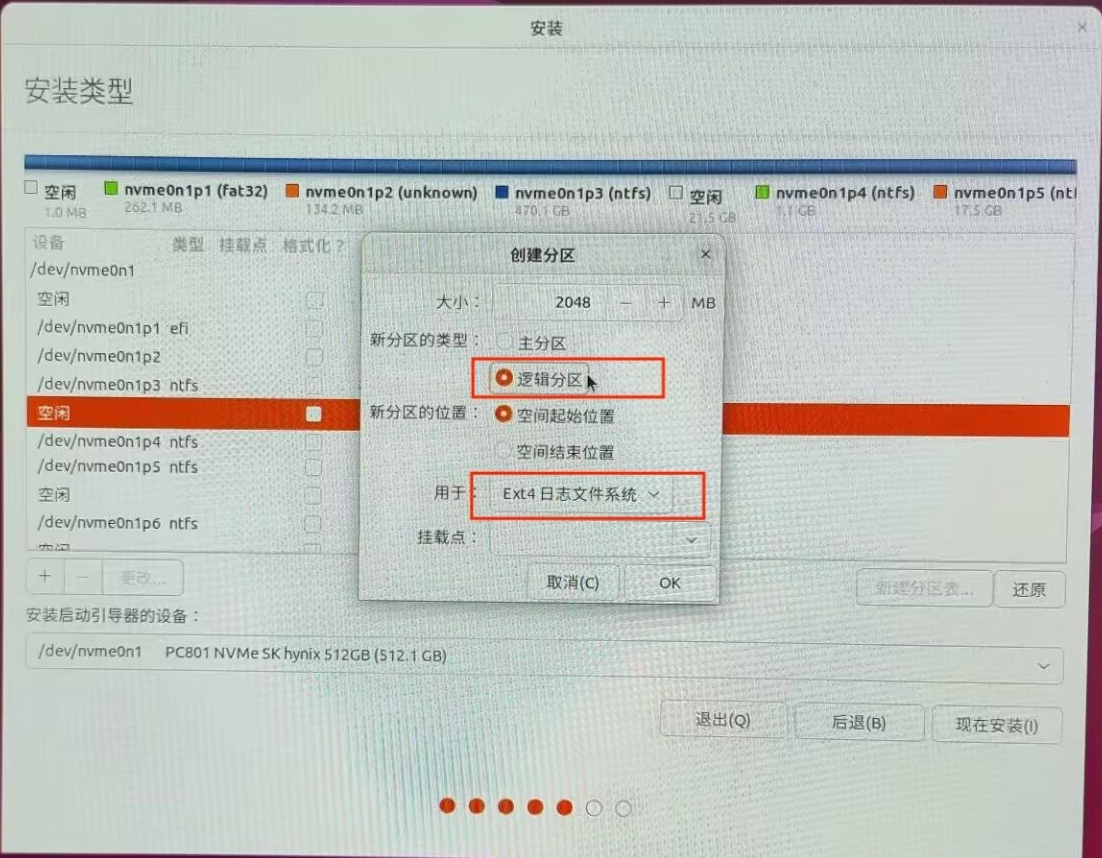
\includegraphics[width=0.7\textwidth]{install5.jpg}
    \caption{分区} % 图片标题
    \label{fig:install5} % 图片标签,用于引用
\end{figure}

再次确定安装启动引导盘的设备选择/boot分区那个路径

\begin{figure}[H]
    \centering
    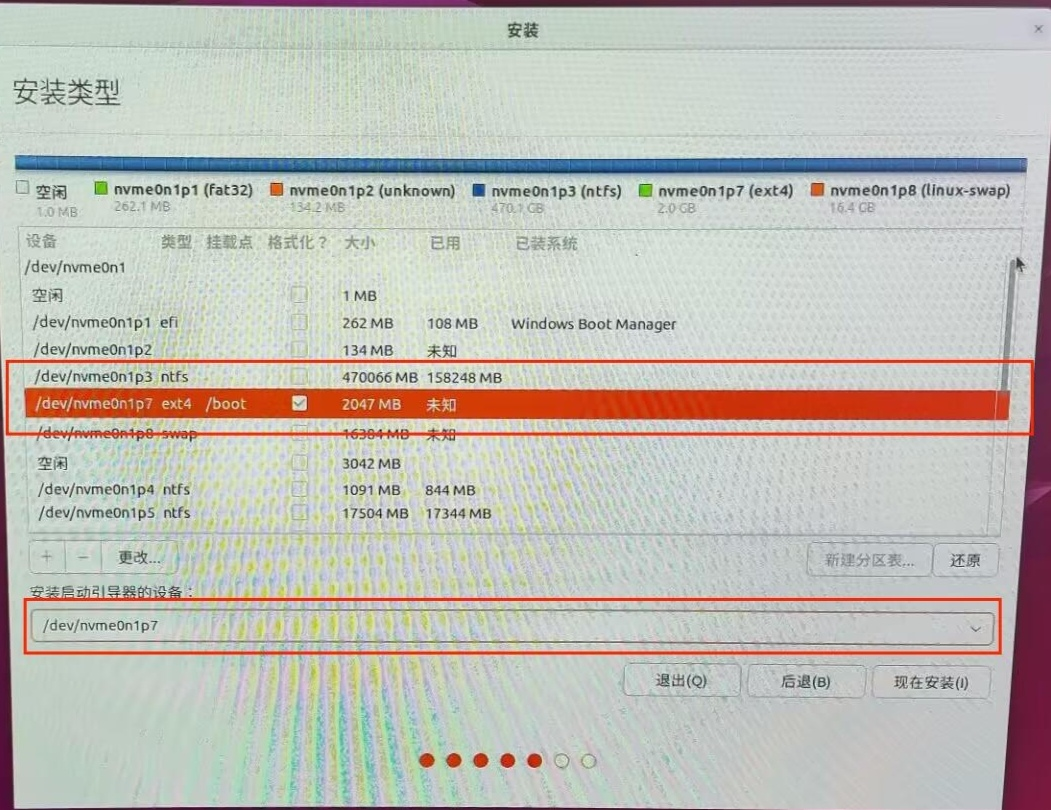
\includegraphics[width=0.7\textwidth]{install6.jpg}
    \caption{安装启动引导盘设备路径} % 图片标题
    \label{fig:install6} % 图片标签,用于引用
\end{figure}

\end{enumerate}
分区完成后点击“现在安装”,选择时区上海就行了。然后填写用户名和计算机密码,如果在上一步中填过了就不需要再填了。

点击“继续”,系统就会对ubuntu系统开始安装了,出现安装完成的提示后点击“现在重启”,等待一会,出现提示“Please remove the installation medium,then press ENTER”后拔掉启动盘并按下ENTER键,进入ubuntu系统的启动引导。在启动页面选择Ubuntu,电脑正常启动后就会进入Ubuntu系统,至此安装就全部完成啦。

ubuntu系统初始是一个什么都没有的状态,但是大家配好了也是可以和windows一样的,接下来各位就按照自己的习惯和喜好进行配置吧。

\subsubsection{系统设置相关}
ubuntu系统安装完成后你的默认启动系统会变成ubuntu,而有的电脑无法通过ubuntu的启动引导进入windows系统,这时候我们要怎样切换回windows系统呢?

首先重启电脑,重启时快速重复按下启动选项快捷键,进入启动引导,在这里选择windows系统即可启动windows。如果常用的系统还是windows,想优先启动windows系统,可以进入BOIS修改启动顺序。进入BIOS依然需要重启电脑,重启时快速重复按下进入BIOS的快捷键,各个主板的快捷键有所不同,可以参考下表进行操作。

\begin{figure}[H]
    \centering
    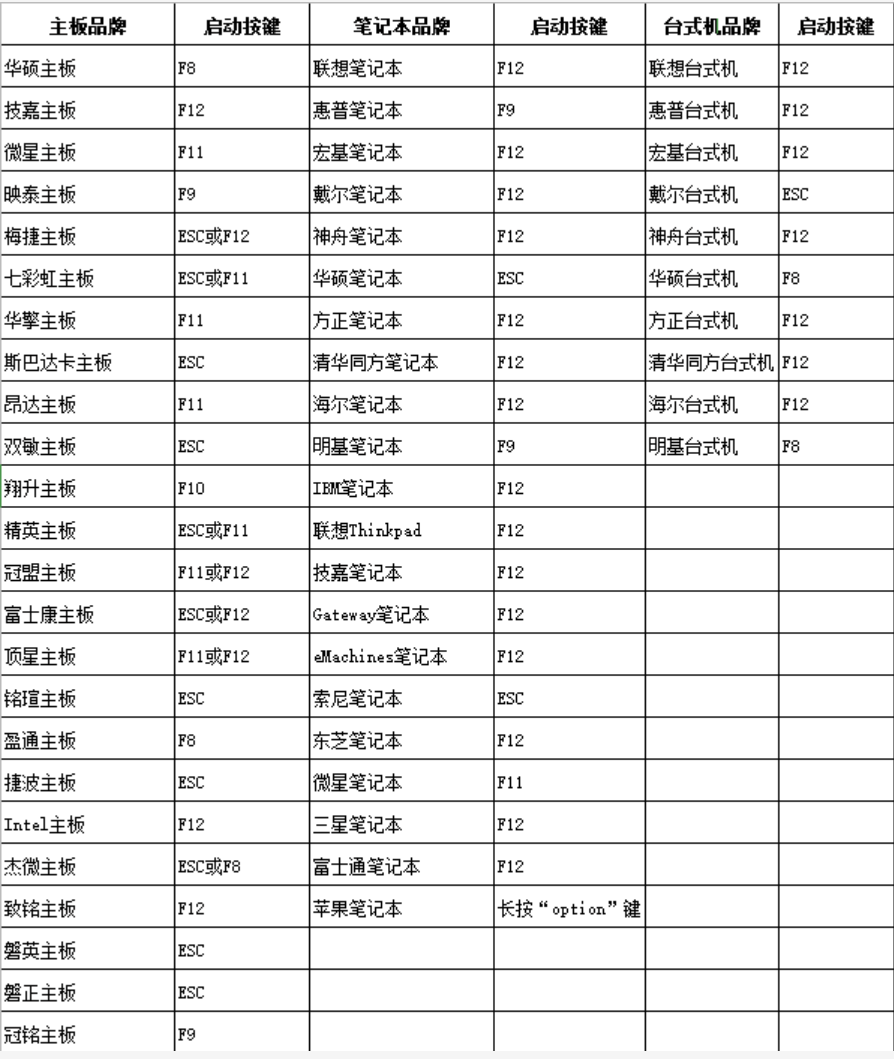
\includegraphics[width=0.7\textwidth]{install7.png}
    \caption{BIOS快捷键一览} % 图片标题
    \label{fig:install7} % 图片标签,用于引用
\end{figure}

进入BIOS后找到Boot相关设置,根据电脑提示将Windows Boot Manager移到ubuntu的启动引导上方,保存退出即可。

既然已经进入了BIOS,还有一点需要注意。如果你的电脑中安装了显卡,那在使用ubuntu之前请在BIOS中将显卡选择为“混合模式”而非“独立显卡”,否则可能出现启动ubuntu后黑屏加载不出来画面的情况。

\subsubsection{系统拓容}

如果系统中的文件已经多到内存爆炸了,那么此时我们就需要给ubuntu系统进行扩容。

扩容使用ubuntu自带的gparted分区管理工具,打开终端,输入

\begin{tcode}
	sudo apt-get install gparted
\end{tcode}

安装完成后输入

\begin{tcode}
	sudo gparted
\end{tcode}

进入gparted图形化界面,可以看到这里显示了电脑中的ubuntu和windows的所有分区,选中你要扩容的ubuntu分区,可以看到上方有一个箭头形状的图标亮起

\begin{figure}[H]
    \centering
    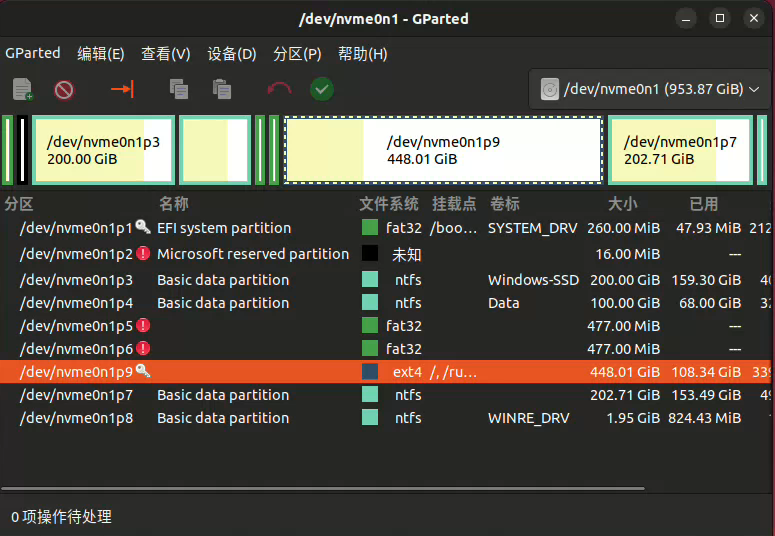
\includegraphics[width=0.7\textwidth]{linux10.png}
    \caption{gparted图形化界面} % 图片标题
    \label{fig:linux10} % 图片标签,用于引用
\end{figure}

点击箭头图标却发现以下报错:

\begin{figure}[H]
    \centering
    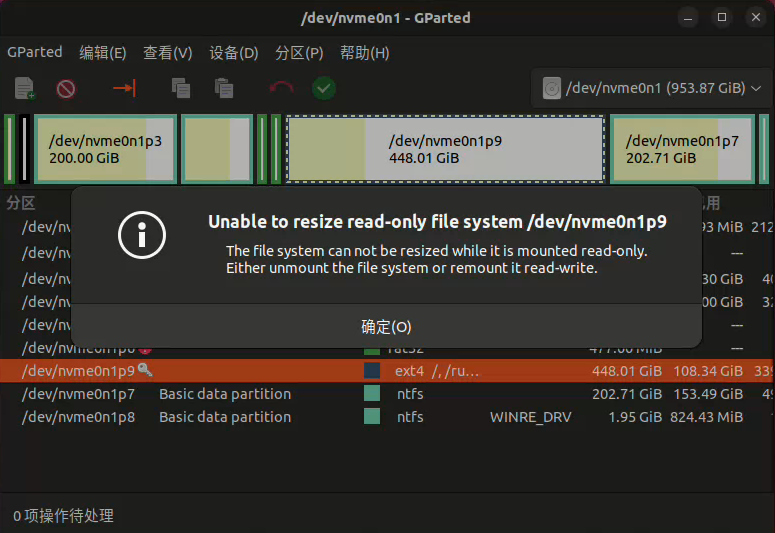
\includegraphics[width=0.7\textwidth]{linux9.png}
    \caption{gparted扩容失败} % 图片标题
    \label{fig:linux9} % 图片标签,用于引用
\end{figure}

这是因为当你处于ubuntu系统时,ubuntu相关的分区是被上锁的,此时你无法对分区进行修改。不过既然在ubuntu系统中不能修改ubuntu的分区,那么切换到别的系统时就可以修改ubuntu的分区。因此我们采取的方法是切换到试用的ubuntu系统再对自己的ubuntu分区进行修改。

在切换之前还有一件事要做:删除linux-swap和extend分区(如果存在的话),这是因为使用gparted扩容时只能对相邻的分区进行操作,如果swap和extend分区挡在ubuntu分区和windows分区之间,那么就不能从这个windows分区中分出内存给ubuntu分区了,因此要先删除这两个分区。

删除之后插上安装ubuntu系统时制作的启动盘,重启电脑,重启时快速重复按下启动选项快捷键。进入启动选项界面后通过上下键选择Linpus lite选项,回车,进入系统安装程序,选择Try or Install Ubuntu,再回车,这些步骤和安装ubuntu时是一样的,只是进入安装页面后,这次我们要选择试用Ubuntu

\begin{figure}[H]
    \centering
    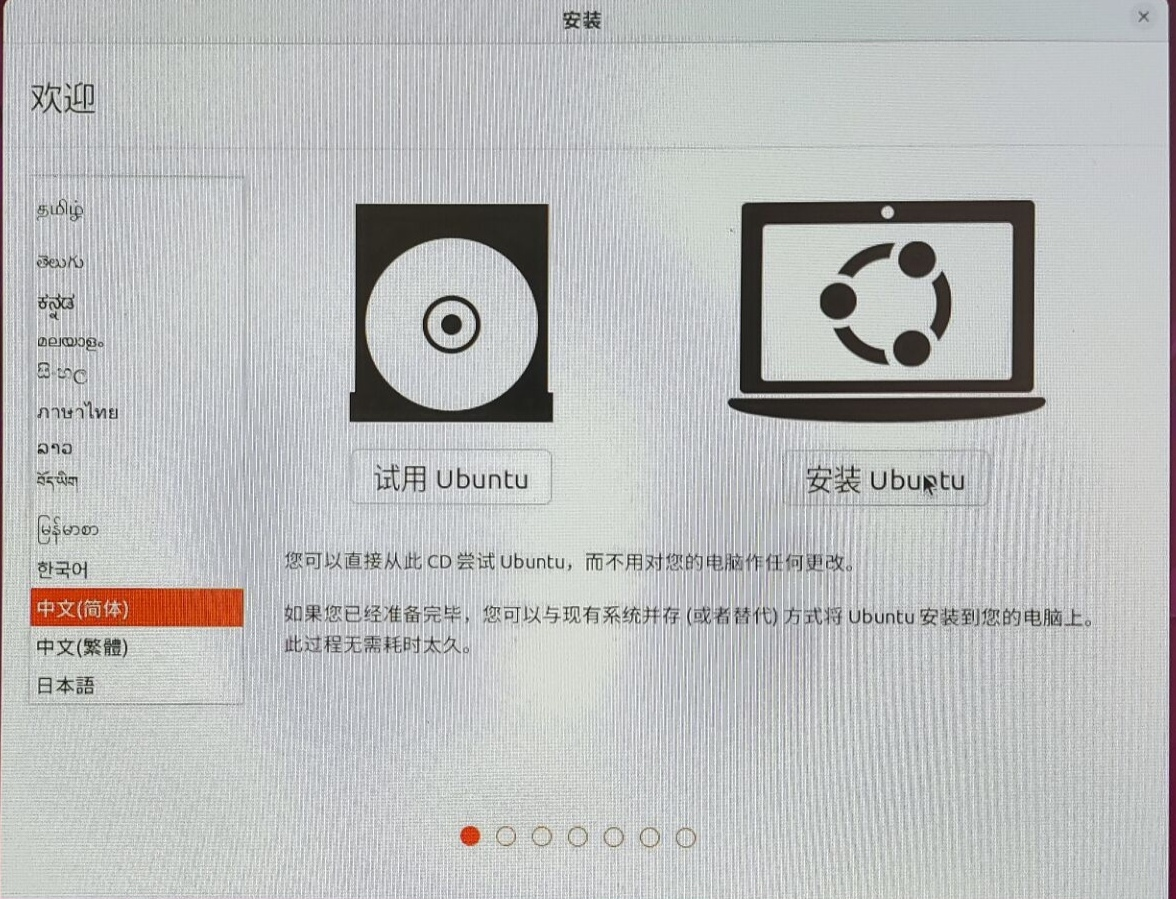
\includegraphics[width=0.7\textwidth]{install2.jpg}
    \caption{进入试用ubuntu界面} % 图片标题
\end{figure}

选择试用后我们会进入到ubuntu的主页面,打开终端,再次打开gparted

\begin{tcode}
    sudo apt-get install gparted
	sudo gparted
\end{tcode}

此时就可以对原来ubuntu系统的分区进行修改了,修改完点击确认等待扩容操作完成即可。